% Template for seminar reports
% Computer Vision Group, Visual Computing Institute, RWTH Aachen University
\documentclass[twoside,a4paper,10pt,DIV=12,BCOR=12mm]{scrartcl}
\usepackage[utf8]{inputenc}    % allows special symbols in LaTeX source code
\usepackage[english]{babel}    % select language of your report (use "ngerman" for German)
\usepackage[T1]{fontenc}       % font encoding, important for umlauts
\usepackage{lmodern}           % lmodern font
\usepackage{xcolor}            % use and define colors for text and images
\usepackage{graphicx}          % include images
\usepackage{booktabs}          % pretty tables
\usepackage{caption}           % captions for figures
\usepackage{subcaption}        % captions for subfigures
\usepackage{url}               % for website links
\usepackage{datetime}          % month on title page
\usepackage{hyperref}          % make references clickable
\usepackage{xspace}            % correct spaces after e.g. "e.g."
\usepackage{tikz}              % custom plots in LaTeX
\usepackage{pgfplots}          % custom function graphs in LaTeX
\usepackage{bm}                % bold math symbols
\usepackage{amsmath}           % additional math environments
\usepackage{amssymb}           % additional math symbols (includes amsfonts)
\usepackage{enumitem}          % change distances for enumerations
\usepackage{listings}          % code
\usepackage{lipsum}            % placeholder text
\usepackage{listings}
\usepackage{color}

\definecolor{dkgreen}{rgb}{0,0.6,0}
\definecolor{gray}{rgb}{0.5,0.5,0.5}
\definecolor{mauve}{rgb}{0.58,0,0.82}

\lstset{frame=tb,
  language=python,
  aboveskip=3mm,
  belowskip=3mm,
  showstringspaces=false,
  columns=flexible,
  basicstyle={\small\ttfamily},
  numbers=none,
  numberstyle=\tiny\color{gray},
  keywordstyle=\color{blue},
  commentstyle=\color{dkgreen},
  stringstyle=\color{mauve},
  breaklines=true,
  breakatwhitespace=true,
  tabsize=3
}

\newdateformat{monthyeardate}{\monthname[\THEMONTH] \THEYEAR}

\setlength{\parindent}{0pt}
\setlength{\parskip}{0pt}
\setlist{nosep}

\makeatletter
\DeclareRobustCommand\onedot{\futurelet\@let@token\@onedot}
\def\@onedot{\ifx\@let@token.\else.\null\fi\xspace}
\def\eg{{e.g}\onedot} \def\Eg{\emph{E.g}\onedot}
\def\ie{{i.e}\onedot} \def\Ie{\emph{I.e}\onedot}
\def\cf{{c.f}\onedot} \def\Cf{\emph{C.f}\onedot}
\def\etc{{etc}\onedot} \def\vs{\emph{vs}\onedot}
\def\wrt{w.r.t\onedot} \def\dof{d.o.f\onedot}
\def\etal{\emph{et al}\onedot}
\makeatother

\overfullrule=1ex

\pgfplotsset{compat=newest}


% =========================================================================

\graphicspath{{pictures/}}
\setcounter{secnumdepth}{3}
\setcounter{tocdepth}{3}

% =========================================================================
\begin{document}

% Template for seminar reports
% Seminar Current Topics in Computer Vision and Machine Learning

\begin{titlepage}
\begin{center}
\ 
\vspace{3.5cm}

\textsf{
RWTH Aachen University \\
Faculty of Mathematics, Computer Science and Natural Sciences\\
Chair of Computer Science 13 (Computer Vision) \\
Prof. Dr. Bastian Leibe
}

\rule{\linewidth}{1pt}

\vspace{1.75cm}
\LARGE
\textbf{Proseminar Report}

\vspace{1.7cm}
\huge
Long Short Term Memory

\vspace{3.0cm}
\Large
Leon Benz\\
\large
Matriculation Number: 445034
\vspace{0.25cm}
\Large
Fynn Jansen\\
\large
Matriculation Number: 467964

\vspace{0.5cm}
\monthyeardate\today

\vspace{1.05cm}
\rule{\linewidth}{1pt}

\vspace{0.5cm}
\textsf{\textbf{
\normalsize
\begin{tabular}{ll}
Advisor:  & name of advisor\\
\end{tabular}
}}
\end{center}

\end{titlepage}


\begin{abstract}

\end{abstract}

\tableofcontents
\newpage
% =========================================================================

\section{Introduction (Fynn)}
Much of the data we encounter in the real world, such as natural language, speech, music and weather, is best described as a sequence of individual data points that must be interpreted in context to extract meaningful information, such as patterns.\\
For instance, individual words do not carry much information and can have multiple meanings depending on the context; however, if multiple words are arranged in a specific order, they can convey complex ideas. Additionally, the order of the words cannot be completely random; it must follow a specific structure to form a proper sentence. This means that, for tasks such as translation, it is important to take the entire context into account in order to properly interpret the meaning of individual words.\cite{harris1954languagestructure}\\
Similarly, most forms of music contain structures and patterns, such as rhythms, chord progressions or melodic motives, which convey meaning; individual notes or transients, on the other hand, convey very little information on their own. Therefore, when writing chord progressions, for example, it is important to consider all previous chords when selecting a chord, as the context will change its sound and meaning.\cite{eck2002musicgeneration}\\
In theory Recurrent Neural Networks can pick up on those patterns, but the algorithms used to train these networks, namely "Back-Propagation Through Time" (BPTT) or "Real-Time Recurrent Learning" (RTRL) had the problem of vanishing or exploding gradients, which made training RNNs impractical, when compared to traditional Feedforward Neural Networks. This problem gets amplified, as the minimum lag between time steps increases.\cite{hochreiter1997lstm,werb1990bptt}\\
The LSTM Architecture, as first described by Sepp Hochreiter and Jürgen Schmidhuber in their 1997 paper, "Long Short-Term Memory" and later refined by Felix A. Gers, Jürgen Schmidhuber and Fred Cummins in their paper "Learning to Forget: Continual Prediction with LSTM" published in 2000, aims to solve some of those issues, by introducing a modified version of the classical RNN structure, to improve the flow of the error signal through the network.\cite{hochreiter1997lstm}\\
Since then, LSTM networks have played a significant role in the development of machine learning-based sequence modeling, most notably in natural language processing, time series forecasting, music generation, and speech recognition.\cite{eck2002musicgeneration,torres2022elctricityforecasting,gers2001timeseries,nielsen2024electricitypriceforcasting, gers2000lstmnlp}\\
\textbf{Outline of Paper.} In Section 2 a few important previous works will be reviewed. Section 3 will cover foundational Concepts, such as Feed Forward Neural Networks ans Recurrent Neural Networks and will examine the problems that lead to the development of the LSTM architecture. Section 4 covers the principle of operation as well as mathematical formalization and implementation of the LSTM architecture.  In Section 5 limitations of the architecture will be examined as well as variations and alternatives, that might resolve some of those problems and section 6 examines possible applications for LSTMs.\\

\section{Previous Work}

\section{Foundational Concepts}

\subsection{Neural Networks and Training}

\subsection{Recurrent Neural Networks}

\subsection{Limitations of Recurrent Neural Networks}

\section{LSTM Architecture}
\subsection{Principle of Operation (Fynn)}
\subsubsection{Intuitive Explanation}
The main goal of the LSTM architecture is to eliminate the problem of vanishing gradients. This can be achieved by ensuring a constant error flow through the network. However, when this approach is implemented naively using only a linear activation function (e.g. \begin{math}f(x)=x,\forall x\end{math}) and a weight matrix with ones on its diagonal (\begin{math}w_{jj}=1,\forall j\end{math}), problems can arise. For the inputs, a single weight can be responsible for both storing and ignoring inputs, and for the outputs, a single weight can be responsible for both allowing and preventing the distribution of a unit's memory. During training, this can result in contradictory weight update signals, affecting the network's performance. \cite{hochreiter1997lstm}\\
The solution proposed by Hochreiter and Schmidhuber introduces so-called 'gate units' at the input and output of the constant error flow to control the storage and retrieval of memory through context. This results in a structure they refer to as a 'memory cell' (often just 'cell'), as shown in Figure \ref{fig:lstm-cell}.\cite{hochreiter1997lstm}.
\begin{figure}[h!]
    \centering
    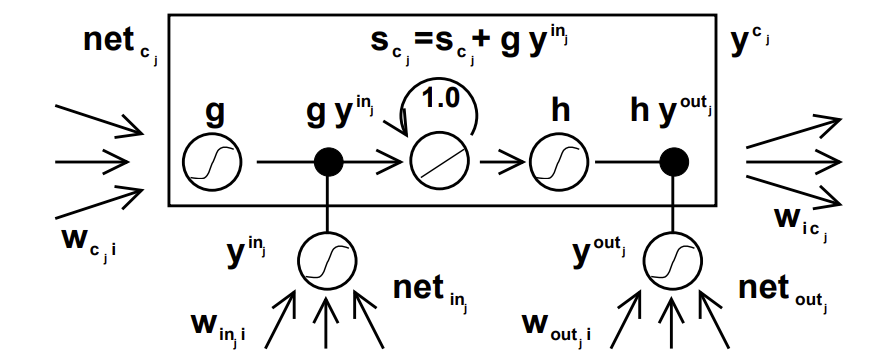
\includegraphics[width=\linewidth]{LSTM-Cell-Diagram.png}
    \caption{LSTM Cell\\ Source: \cite{hochreiter1997lstm}}
    \label{fig:lstm-cell}
\end{figure}
\\As their name suggests, gate units are used to restrict the flow of information.  The amount of gating applied to an input is determined by values computed from another input, enabling the gate to open and close depending on the context. Figure \ref{fig:lstm-cell} shows input and output gates represented by large black dots inside the cell, where input flows from left to right through the gate and control input reaches the gate from the bottom.\cite{hochreiter1997lstm}
Internally, the cell stores a state which normally starts at \begin{math}0\end{math} and to which the scaled input is added. This state is then scaled using the activation of the output gate to compute the output.
This means that an LSTM cell comprises three individual parts:\\
\textbf{Input Gate.} The input gate. The input gate controls how much of the cell's input should be stored in memory, thereby determining which inputs are relevant. in the given context.\\
\textbf{Internal State.} The internal state can be viewed as the cell's memory. It is computed using the state from the previous time step to which the cell input activations, after scaling using the input gate activations are added.\\
\textbf{Output Gate.} The output gate scales the cell state before output, thereby controlling the retrieval of information from the cell.\cite{hochreiter1997lstm} \\
To improve understanding of how information flows through an LSTM cell, let us follow the flow of information through the cell at a single time step:
First, the net input for the cell and the gates is computed by multiplying the weights by the inputs (for example, the current activations of the input units and the previous output activations of the cell) and summing them. Next, the activation functions are evaluated on the gate net input activations to compute the gate activations. Then the cell net input is scaled using a function, and then scaled again using the input activations. This result is then added to the internal state to update it. Finally,  the internal state is scaled using another function, then scale each component using the output gate activations to obtain the cell output activations.\cite{hochreiter1997lstm}
\subsubsection{Mathematical Formalization}
To formalize this approach, the activations at time t are defined as the output of the respective activation function of the net input at that time:\\
\textbf{Input gate activations:}
\begin{equation}
\label{eqn:poo-act-in}
y^{in}(t)=f_{in}\left(net_{in}(t)\right).
\end{equation}
\textbf{Output gate activations:}
\begin{equation}
\label{eqn:poo-act-out}
y^{out}(t)=f_{out}\left(net_{out}(t)\right)
\end{equation}
\textbf{Cell output activations:}
\begin{equation}
\label{eqn:poo-act-c}
y^{c}(t)=y^{out}(t)h\left(s_c(t)\right)
\end{equation}
where \begin{math}s_c\end{math} is the "internal state" of the cell, given by:
\begin{equation}
\label{eqn:poo-state0}
s_c(0)=0
\end{equation}
\begin{equation}
\label{eqn:poo-state}
s_c(t)=s_c(t-1)+y^{in}(t)g\left(net_c(t)\right)
\end{equation}
and the net inputs \begin{math}net_{in}(t), net_{out}(t)\end{math} and \begin{math}net_c(t)\end{math} are the sum of the result of multiplying the weight matrix with the activations from the previous time step for all different inputs:\\
\textbf{Input gate net input:}
\begin{equation}
\label{eqn:poo-net-in}
net_{in}(t)=\sum_{u}{w_{in\ u}}y^u(t-1).
\end{equation}
\textbf{Output gate net input:}
\begin{equation}
   \label{eqn:poo-net-out}
   net_{out}(t)=\sum_{u}{w_{out\ u}}y^u(t-1).
\end{equation}
\textbf{Cell net input:}
\begin{equation}
   \label{eqn:poo-net-c}
   net_{c}(t)=\sum_{u}{w_{c\ u}}y^u(t-1).
\end{equation}
The values of the summation index \begin{math}u\end{math} represent the different inputs and depend on the chosen network architecture. These values can represent input units, memory cells, gate units, or hidden units from this or other cells.
The function \begin{math}g\end{math} is used to scale the cell net input before gating, and the function \begin{math}h\end{math} is used to scale the memory cell output before gating.
Note that multiplying two vectors together does not give the dot product, but rather the Hadamard product, which multiplies vectors component-wise.\cite{gokmen2018hadamard} This allows each component of the vector to be gated individually.
An index \begin{math}j\end{math} can be added to identify individual cells. This has been omitted here to make the notation easier to read.\cite{hochreiter1997lstm}

\subsection{Example Implementation (Fynn)}
\subsubsection{Network Architecture}
Before implementing a simple LSTM network, the network architecture must first be defined.
For simplicity, the activations for the cell, input gate and output gate will be the output activations, as well as the activations of the input units:   \begin{math}u\in\{c, x, b \}\end{math}, where \begin{math}y^c(t)\end{math} are the output activations at time \begin{math}t\end{math}, \begin{math}y^x(t-1)=x(t)\end{math} are the activations of the input units at time \begin{math}t\end{math} and \begin{math}y^b(t-1)=b\end{math} are the bias units.\\\cite{hochreiter1997lstm} 
As the biases are constant we can define \begin{math}b_u=w_{u\ b}b\end{math} and use those individual biases as weights to reduce the total number of weights.
This means that the sums describing the inputs for the input gate, output gate and cell  (see equations \ref{eqn:poo-net-in}, \ref{eqn:poo-net-out}, and \ref{eqn:imp-net-c})  an be written as follows:
\begin{equation}
\label{eqn:imp-net-in}
net_{in}(t)=w_{in\ c}y^c(t-1)+w_{in\ x}x(t)+b_{in},
\end{equation}
\begin{equation}
\label{eqn:imp-net-out}
net_{out}(t)=w_{out\ c}y^c(t-1)+w_{out\ x}x(t)+b_{out}
\end{equation}
\begin{equation}
\label{eqn:imp-net-c}
net_c(t)=w_{c\ c}y^c(t-1)+w_{c\ x}x(t)+b_c.
\end{equation}
\subsubsection{Implementing the Network}
The PyTorch library is used for the implementation of the network. To keep things simple, the input and output will always be vectors of the same length given by the parameter \lstinline{size}.\\
Firstly, a class that extends \lstinline{torch.nn.Module} s defined, along with its attributes: the input/output size of the cell; the weight matrices \begin{math}w_{in\ c},w_{in\ x},w_{out\ c},w_{out\ x},w_{c\ c},w_{c\ x}\end{math}; and the biases \begin{math}b_{in},b_c,b_{out}\end{math}:\cite{keras-lstm,pytorch-lstm}
\begin{lstlisting}
class LSTMCell(torch.nn.Module):
    
    size : int # Input Size (1D)
    
    w_i_c : torch.Tensor # Input gate weights
    w_i_x : torch.Tensor # Input gate weights
    w_c_c : torch.Tensor # Cell input weights
    w_c_x : torch.Tensor # Cell input weights
    w_o_c : torch.Tensor # Output gate weights
    w_o_x : torch.Tensor # Output gate weights
    
    b_i : torch.Tensor # Input gate biases
    b_c : torch.Tensor # Cell input biases
    b_o : torch.Tensor # Output gate biases
\end{lstlisting}
When a new object of the class is created, the weights should be randomized, as shown in (a), and the biases should be initialized to zero, as shown in (b). All of these should also be marked as trainable parameters, which can be achieved by using \lstinline{torch.nn.Parameter}:\cite{keras-lstm,pytorch-lstm}
\begin{lstlisting}
def __init__(self, size : int):
    super(LSTMCell, self).__init__()
    self.size = size
    
    # Initialize weights (a)
    self.w_i_c = torch.nn.Parameter(torch.randn(size, size) * 0.01)
    self.w_i_x = torch.nn.Parameter(torch.randn(size, size) * 0.01)
    self.w_c_c = torch.nn.Parameter(torch.randn(size, size) * 0.01)
    self.w_c_x = torch.nn.Parameter(torch.randn(size, size) * 0.01)
    self.w_o_c = torch.nn.Parameter(torch.randn(size, size) * 0.01)
    self.w_o_x = torch.nn.Parameter(torch.randn(size, size) * 0.01)
    
    # Initialize weights biases (b)
    self.b_i = torch.nn.Parameter(torch.zeros(size))
    self.b_c = torch.nn.Parameter(torch.zeros(size))
    self.b_o = torch.nn.Parameter(torch.zeros(size))   
\end{lstlisting}
Next, the activation functions are defined based on those used in the Hochreiter and Schmidhuber experiments. The functions\begin{math}f, g\end{math} and \begin{math} h \end{math} are given as follows: \cite{hochreiter1997lstm}
\begin{equation}
    \label{eqn:imp-f}
    f(x)=\frac{1}{1+\exp(-x)},
\end{equation}
\begin{equation}
\label{eqn:imp-g}
    g(x)=\frac{4}{1+\exp(-x)}-2
\end{equation}
\begin{equation}
    \label{eqn:imp-h}
    h(x)=\frac{2}{1+\exp(-x)}-1.
\end{equation}
For function \begin{math}f\end{math} (see \ref{eqn:imp-f}, \lstinline{torch.sigmoid} is used, as it is a standard sigmoid function. The functions \begin{math}g\end{math} and \begin{math}h\end{math} (see \ref{eqn:imp-g}, \ref{eqn:imp-h}) are just scaled and shifted sigmoid functions, they can be implemented by multiplying the result of the sigmoid function with a scalar, and subtracting a tensor of the same shape as the input, set to either \begin{math}1\end{math}'s (see (c)) or \begin{math}2\end{math}'s (see (d)) entirely:\cite{hochreiter1997lstm, pytorch-lstm}
\begin{lstlisting}
@staticmethod
def _f(x: torch.Tensor) -> torch.Tensor:
    return torch.sigmoid(x)
@staticmethod
def _g(x: torch.Tensor) -> torch.Tensor:
    return torch.sigmoid(x) * 4 - torch.ones_like(x) * 2 # (c)
@staticmethod
def _h(x: torch.Tensor) -> torch.Tensor:
    return torch.sigmoid(x) * 2 - torch.ones_like(x) # (d)
\end{lstlisting}
These can then be used to implement a function that forwards an input through the cell. This function takes the current input, as well as the cell's previous output and state, and returns the cell's output and current state. To compute the outputs, the input \lstinline{x_t} must first be converted to a vector if it is a scalar (see (e)), so that the matrix multiplication operator can be used in the case \lstinline{size == 1}:\cite{keras-lstm, pytorch-lstm}
\begin{lstlisting}
def forward(self, x_t : torch.Tensor, y_tm1 : torch.Tensor, c_tm1 : torch.Tensor) -> tuple[torch.Tensor, torch.Tensor]:
    if x_t.dim() == 0:  # x_t is scalar (e)
        x_t = x_t.unsqueeze(0)
\end{lstlisting}
Using equations \ref{eqn:imp-net-in} and \ref{eqn:imp-net-out}, the net input for the input, as well as the input and output gates, can be calculated, as shown at (f) and (h). This can then be passed through the function f (see equation \ref{eqn:imp-f}) to obtain the respective gate activations, as shown at (g) and (i) (see equation  \ref{eqn:poo-act-in} and \ref{eqn:poo-act-out}):\cite{hochreiter1997lstm, keras-lstm, pytorch-lstm}
\begin{lstlisting}
# Input gate activations
net_i = self.w_i_c @ y_tm1 + self.w_i_x @ x_t + self.b_i # (f)
y_i   = self._f(net_i)                                   # (g)
        
# Output gate activations
net_o = self.w_o_c @ y_tm1 + self.w_o_x @ x_t + self.b_o # (h)
y_o   = self._f(net_o)                                   # (i)
\end{lstlisting}
Using those, the cell net input is computed using equation \ref{eqn:imp-net-c} as is implemented at (j). 
The cell state is computed using equation \ref{eqn:poo-state} as is done at (k) and the cells output using equation \ref{eqn:poo-act-c} as is done at (l). Finally the output and cell state are returned, for the next time step:\cite{hochreiter1997lstm,keras-lstm, pytorch-lstm}:
\begin{lstlisting}
# Compute cell input
net_c = self.w_c_c @ y_tm1 + self.w_c_x @ x_t.squeeze() + self.b_c # (j)
c_t = c_tm1 + y_i * self._g(net_c) # Update cell state               (k)
y_t = y_o * self._h(c_t)           # Compute output                  (l)
        
return y_t, c_t
\end{lstlisting}
\subsubsection{Testing the implementation}
To test whether the implementation works, two LSTM cells are created: one with a size of 1 and one with a size of 20. An input matching the size of each cell is then passed through them:\cite{pytorch-lstm}
\begin{lstlisting}
lstm1 = LSTMCell(1)
lstm1(torch.zeros(1), torch.zeros(1), torch.zeros(1)) # x_t, y_tm1, c_tm1
lstm20 = LSTMCell(20)
lstm20(torch.zeros(1), torch.zeros(1), torch.zeros(1))
\end{lstlisting}
This code executes without throwing any errors, implying that all the tensors are the intended size and that there are no other critical errors in the implementation.\\
Next, the performance is tested on a sequence of values sampled from the function \begin{math}\sin(2\pi t)\end{math}. 
First, the function for generating the sequence is defined with parameters for noise and sample lag. This outputs a list containing two elements: the sampled value and the time difference to the previous value. This time difference is constant if no sampling lag is applied:
\begin{lstlisting}
def genSequence(length : int, dt : float = 0.05, noise = 0, samplingLag = 0) -> list[list[float]]:
    t = 0
    result = []
    for i in range(length):
        tm1 = t
        t = t + dt + samplingLag * random.uniform(-1, 1) * dt
        x = math.sin(2 * math.pi * t) + noise * random.uniform(-1, 1)
        result.append([x, t - tm1])
    return result
\end{lstlisting}
The model is defined, as an LSTM cell with a size of 2. The loss function chosen is Mean Absolute Error, as it is typically used for regression tasks like this and so the loss of errors \begin{math}<1\end{math} is not squished and ADAM is chosen as the optimizer, as it works well for LSTMs:\cite{chang2018adamlstm,willmott2005losses,terven2025losses}
\begin{lstlisting}
model = LSTMCell(2)
loss_fn = torch.nn.L1Loss()  # L1Loss for regression tasks 
optimizer = torch.optim.Adam(model.parameters(), lr=0.0015)
\end{lstlisting}
Finally, the train function can be implemented:
\begin{lstlisting}
def train(epochs : int, batches : int, batch_size : int):
    data = genSequence(batch_size * batches, samplingLag=0.0, noise=0.0)
    for epoch in range(epochs):
        total_loss = 0.0
        for n in range(batches):
            # Zero gradient and batch_loss (m)
            optimizer.zero_grad() 
            batch_loss = 0.0
            
            # Get batch data # (n)
            batch = torch.tensor(data[n * batch_size : (n + 1) * batch_size])    
            # Initialize internal state and input (o)
            c_t = torch.zeros(model.size)
            y_t = torch.zeros(model.size)
            
            # Compute output and loss for each time step and add up all the losses (p)
            for t in range(batch_size - 1):
                input = batch[t]
                target = batch[t + 1]
                y_t, c_t = model(input, y_t, c_t)
                loss = loss_fn(y_t[0], target[0])
                batch_loss += loss      
            # Calculate the average the batch loss and backpropogate it (q)
            batch_loss /= (batch_size - 1)  # Average loss for the batch
            total_loss += batch_loss.item()
            batch_loss.backward()
            
            # Gradient clipping, to avoid expoloding gradients
            # and adjust parameters (r)
            torch.nn.utils.clip_grad_norm_(model.parameters(), 1.0)
            optimizer.step() 
        avg_loss = total_loss / batches
        print(f"Epoch {epoch + 1}/{epochs}, Average Loss: {avg_loss:.4f}")
        loss_graph.gca().plot(epoch, avg_loss, 'ro')
\end{lstlisting}
\begin{figure}[h!]
    \centering
    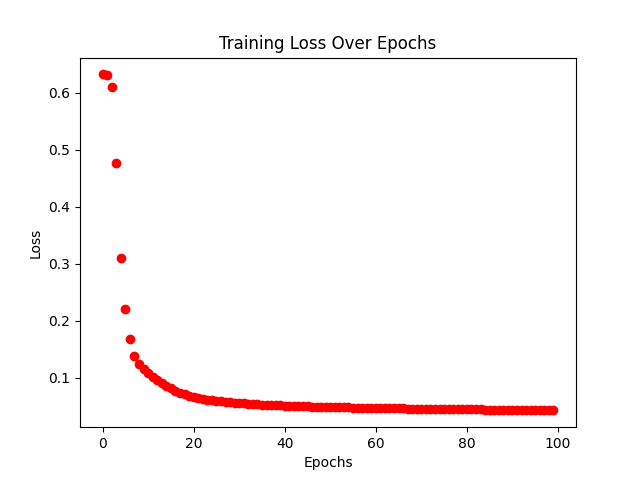
\includegraphics[width=0.75\linewidth]{train_loss_graph.png}
    \caption{Training loss}
    \label{fig:train-loss-graph}
\end{figure}
The function first generates a Sequence, then trains the network on all batches for the specified number of epochs. For each batch the first step is to zero the gradient and batch loss as done at (m). Next the batch is retrieved from the sequence and converted to a tensor as done at (n). Then the internal state is set to zero, as required by Equation \ref{eqn:poo-state0} and the cell's current output is set to zero as well as done at (o). Next, the output and loss at each time step are computed and summed up for each time step, as is done at (p). This is archived, by passing each input in the batch into the network and updating the cell state and the cell output, so they can be used as inputs at the next time step. Afterwards the average of the batch is calculated by dividing by the batch size, and this average gets back-propagated through the network, as is done at (q). Finally at (r), the gradients are clipped, to avoid exploding gradients, and the models parameters are adjusted. An average of the current batch loss is also computed, which is printed for monitoring training, and added to a plot for visual analysis.\cite{werb1990bptt, pytorch-rnn, gradient-clipping, pascanu2013rnntraining, hochreiter1997lstm}  
\\Training the network for 100 epochs, with 100 batches of size 125 each, results in the graph Figure \ref{fig:train-loss-graph}, which shows a typical curve for training a neural network, with a steep drop off at the start, which then settles to a value.\cite{training-graphs}
The decrease in the loss function indicates successful training. Due to the L1Loss, the Average Loss is \begin{math}\ell_a=\overline \ell_b\end{math} where the average batch loss \begin{math}\ell_b=\overline{\left|d(t)-y^c(t)\right|}\end{math}, meaning it is the average of the average batch loss over all batches, where the average batch loss is the average of the absolute value of the difference between expected output and the networks output. Because the loss is directly proportional to the difference between target and output, small and large errors are weighted equally in training.\\
Now the network is tested by predicting a sequence with different lengths. For this a sequence is first generated, the  cell state and cell output initialized with zero, and then the network is called and the loss computed similarly as to how it was done when training the network:
\begin{lstlisting}
seq, y_t, c_t = genSequence(25), torch.zeros(model.size), torch.zeros(model.size)
for t in range(0, 24):
    x_t = torch.tensor(seq[t])
    y_t, c_t = model(x_t, y_t, c_t)
    test_graph.gca().plot(t, loss_fn(y_t[0], torch.tensor(seq[t+1][0])).item(), 'bo')
\end{lstlisting}

\begin{figure}[h!]
    \centering
    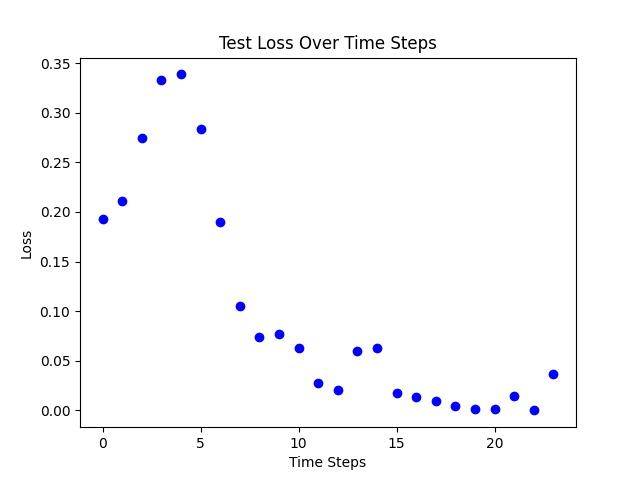
\includegraphics[width=0.75\linewidth]{test_loss_graph.png}
    \caption{Test sequence loss}
    \label{fig:test-loss-graph}
\end{figure}
The loss at each timestep is added to the plot shown in Figure \ref{fig:test-loss-graph}. The plot clearly shows that the network struggles to predict the next value for short input sequences, but its performance improves as the sequence gets longer, which is typical for LSTMs. \cite{bolboaca2023lstmperformance} Overall, the predicted values never deviate by more than \begin{math}0.35\end{math} from the targets.\\
Next, the performance is tested with noise and sampling lag added by simply adjusting the \lstinline{noise} and \lstinline{samplingLag} parameters in the train function and test sequence.
\begin{figure}[h!]
    \centering
    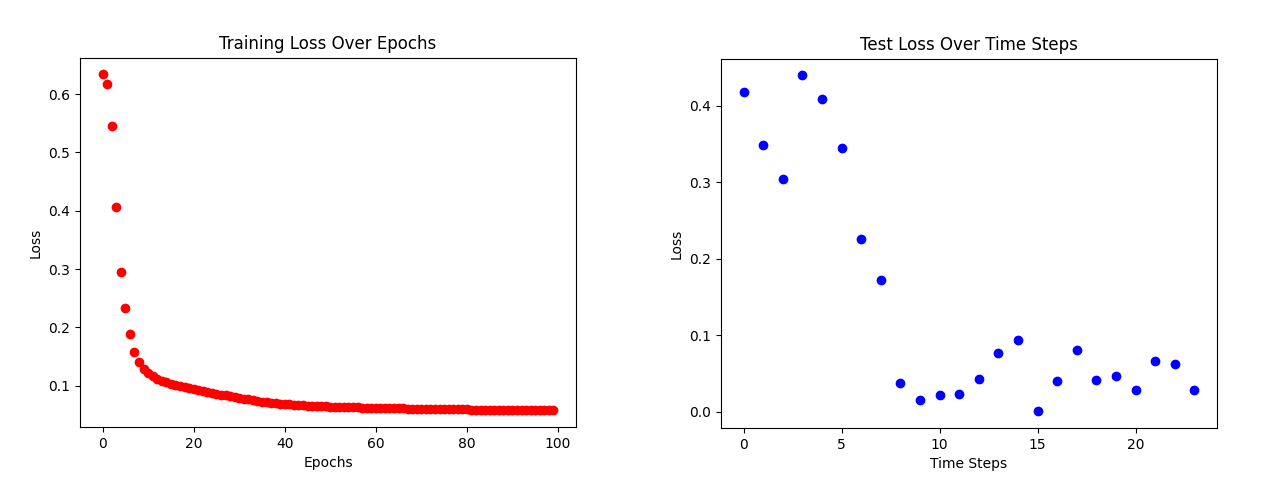
\includegraphics[width=\linewidth]{loss_with_noise.png}
    \caption{Losses with 10\% sampling lag and 5\% noise added to data}
    \label{fig:loss-noise}
\end{figure}
\\The resulting graphs, shown in Figure \ref{fig:loss-noise}, demonstrate that the model's performance is only slightly worse than on data with no noise. The loss during training settles at a slightly higher value and the loss during testing is about \begin{math}0.1\end{math} higher for short sequences and  \begin{math}0.05\end{math} higher for longer sequences.\\
\textbf{Possible Improvements:}
As the input is a repeating sequence of values, the implementation could be improved by introducing a forget gate. This would allow the network to predict the next values without needing to consider the entire previous sequence.\cite{forget-gate}\\
Another way to get a better performance would be to use a Gated recurrent unit (GRU) instead of an LSTM, as GRUs often perform better with short sequences.\cite{cahuantzi2023lstmvsgru}
\section{Limitations and Alternatives}

\subsection{Limitations (Fynn)}
Although LSTMs solve some of the problems associated with classical RNNs, they also have some disadvantages, including:
\begin{itemize}
    \item \textbf{Computational Intensity:} Computational intensity: As an LSTM cell requires additional weights for the gates, the number of weights can increase by up to a factor of \begin{math} 9 \end{math}. However, this is usually not a significant issue, as LSTM networks typically have a similar number of weights to other RNNs.\cite{hochreiter1997lstm}\\ However, in applications that require low power, such as mobile devices, this could cause problems. \cite{rizakisFPGAlstm}
    \item \textbf{Exploding Gradients:} Although the LSTM architecture mitigates the issue of vanishing gradients, it does not eliminate that of exploding gradients.\cite{pascanu2013rnntraining} This can be achieved using alternative techniques, such as gradient clipping.\cite{gradient-clipping, pascanu2013rnntraining}
    \item \textbf{Limited GPU utilization and memory bottlenecks:} LSTM networks do not utilise the GPU fully and tend to train less efficiently on modern GPUs. Furthermore, they are often limited by the available GPU memory.\cite{zheng2018scalability, zheng2020scalability}  
    \item \textbf{Worse performance on less complex sequences:} Although LSTMs perform better than some other architectures, such as GRUs, on sequences with high complexity, they struggle more on simpler sequences.\cite{cahuantzi2023lstmvsgru} 
    \item \textbf{Worse performance on short sequences:} As discussed in Section 4.2.3, LSTMs tend to perform poorly with short sequences, often achieving significantly higher loss. \cite{bolboaca2023lstmperformance} 
\end{itemize}

\subsection{Variants}

\subsubsection{LSTM with Forget Gate (Fynn)}
\begin{figure}
    \centering
    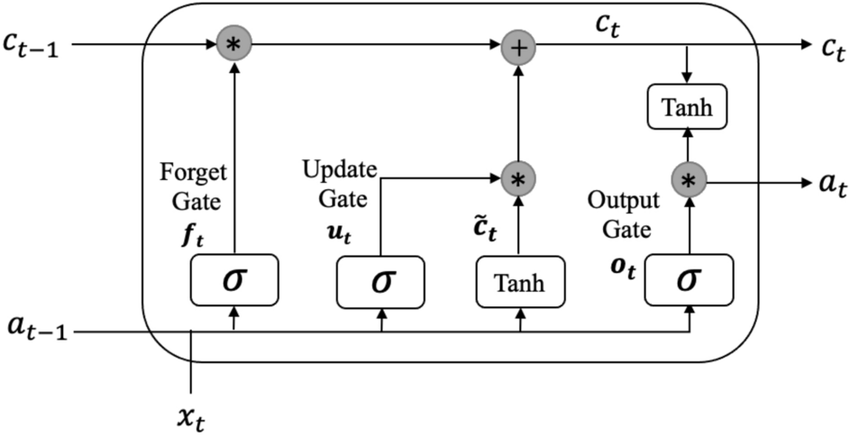
\includegraphics[width=0.75\linewidth]{Structure-of-LSTM-cell-which-introduces-three-special-gates-Input-Gate-i-Forget-Gate.png}
    \caption{LSTM Cell with forget gate\\ Source: \cite{nguyen2022lstmforgetgraphic}}
    \label{fig:lstm-forget}
\end{figure}
One of the first variations of Hochreiters and Schmidhubers architecture, was the introduction of a forget gate. The reason for its introduction, is that there is no way for the internal state of the cell to be reset in the original architecture. To fix this a forget gate can be introduced, which restricts how much of the previous state is kept in the next time step.\cite{gers1999forgetgate}
Figure \ref{fig:lstm-forget} shows an LSTM cell, with the added forget gate on the left of the cell. Note that the input gate is labeled as update gate in this graphic.\\
The forget gate is implemented like the other with\cite{gers1999forgetgate}
\begin{equation}
    net_\varphi(t)=\sum_uw_{\varphi\ u}y^u(t-1)
    \label{eqn:forget-net-in}
\end{equation}
and
\begin{equation}
    y^\varphi(t)=f_\varphi\left(net_\varphi(t)\right)
    \label{eqn:forget-actiavtions}
\end{equation} 
Equation \ref{eqn:forget-net-in} describes the net inputs for the forget gate, and equation \ref{eqn:forget-actiavtions} describes the activation for the forget gate. Using those a new equation for the cell state can be defined as\cite{gers1999forgetgate}
\begin{equation}
    s_c(t)=y^\varphi(t)s_c(t-1)+y^{in}(t)g\left(net_c(t)\right).    
\end{equation}
  This addition is very common, and many LSTM implementations in commonly used machine learning frameworks, include a forget gate.\cite{keras-lstm, pytorch-lstm}
 \subsubsection{Coupled Input-Forget Gate}

\subsubsection{Simplified LSTM}

\subsubsection{LSTM with Attention}

\subsubsection{Bidirectional LSTM}

\subsubsection{Deep LSTM}

\subsubsection{Zoneout LSTM}

Examines notable variants discussing their respective enhancements and capabilities.
(Approximately 1-1.5 pages, written by Leon/Fynn)

\subsection{LSTM vs GRU}

\subsection{LSTM vs Transformers}

\section{Applications}

\subsection{Natural Language Processing}

\subsection{Time Series Forecasting (Fynn)}
While LSTMs can be used to forecast timeseries, they often are inferior to other methods.\cite{gers2001timeseries} But for certain applications, like speech or music, they are a better choice, as they perform better on more complex sequences.\cite{gers2001timeseries, cahuantzi2023lstmvsgru}\\
In a 2022 article by Torres, they use an Deep LSTM Network, to predict electricity demands, and archive errors of just \begin{math}1.5\%\end{math}.\cite{torres2022elctricityforecasting}\\
Kılıç et al. (2024) uses the LSTM Architecture, to predict electricity prices, and archieve better results compared to other architectures.\cite{nielsen2024electricitypriceforcasting}

\subsection{Music and Audio (Fynn)}
As mentioned in the introduction, music has structures and patterns, where the next note or chord, depends on the previous ones. LSTMs can learn those patterns and predict what comes next, which allows them to generate music.\cite{eck2002musicgeneration}\\
In their 2002 paper Eck and Schmidhuber use an LSTM network to generate chord progressions, as well as melodies and chord progression. Their network successfully managed to pick up on patterns in a style of music, and reproduce those patterns to compose new music in they same style.\cite{eck2002musicgeneration}  
\subsection{Medical}

\section{Conclusion}

Summarizes the relevance of LSTM networks, reflecting on current applications and potential future directions.
(Approximately 0.5 pages, written by Fynn)

\bibliographystyle{alpha}
\bibliography{abbrev,seminar_report}
\end{document}